\section{Michelson干渉計}

Michelson干渉計は、2本の腕を往復した光の位相差を干渉信号として出力する装置である。


\subsection{重力波の応答}
$+$モードの重力波がMichelson干渉計平面に垂直なZ軸方向から入射,つまり歪みテンソル$h_{\mu\nu}$が
\begin{equation}
  h_{\mu\nu} =
  \left(
  \begin{array}{cccc}
    -c^2 & 0      & 0      & 0 \\
    0   & 1+h(t) & 0      & 0 \\
    0   & 0      & 1-h(t) & 0 \\
    0   & 0      & 0      & 1 
  \end{array}
  \right)  
\end{equation}
となって時空を歪ませる場合を考える。

Michelson干渉計は2本の腕の位相差を測る装置なので、それぞれのアームを往復して生じる位相遅れ、$\phi_{x}$と$\phi_{y}$をもとめる。さて、光は$ds^2 = h_{\mu\nu}dx^{\mu}dx^{\nu} = 0 $の世界線に沿うので、例としてXアームの場合は
\begin{eqnarray}\label{eq:eq2}
  dx = \frac{c}{\sqrt{(1+h(t))}}dt
\end{eqnarray}
という条件をみたしながらレーザー光はXアームを走る。式(\ref{eq:eq2})の両辺を積分すると
\begin{eqnarray}\label{eq:eq3}
{2l_x} = \int dx &=& \int_{t-\tau_{x}}^{t} \frac{c}{\sqrt{(1+h(t^{\prime}))}}\, dt^{\prime} \simeq \int_{t-\tau_{x}}^{t} c\left(1-\frac{1}{2}h(t^{\prime})\right) \,dt^{\prime}
\end{eqnarray}
となる。$\tau_x$は往復にかかった時間である。式(\ref{eq:eq3})を$\tau_x$について解くと,$\tau_x$は
\begin{eqnarray}\label{eq:eq4}
  \tau_{x} &=& \frac{2l_x}{c} - \frac{1}{2}\int_{t-\tau_{x}}^{t} h(t^{\prime})\, dt^{\prime} \simeq \frac{2l_x}{c} - \frac{1}{2}\int_{t-l_{x}/c}^{t} h(t^{\prime})\, dt^{\prime}  
\end{eqnarray}
と表すことができる。ここで,$h(t)\ll1$なので$\tau_{x}\sim 2l_x/c$という近似をした。
したがって,往復したあとのレーザー光の位相遅れは,
\begin{eqnarray}\label{eq:eq5}
  \phi_{x} = \omega_{0}\tau = \frac{2\omega_{0}l_x}{c} - \frac{\omega_{0}}{2}\int_{t-l_{x}/c}^{t} h(t^{\prime})\, dt^{\prime}  
\end{eqnarray}
となる。一方でyアームを往復して遅れる位相は,h(t)の符号に注意して,同様の計算をすれば
\begin{eqnarray}\label{eq:eq6}
  \phi_{y} =  \frac{2\omega_{0}l_y}{c} - \frac{\omega_{0}}{2}\int_{t-l_{y}/c}^{t} h(t^{\prime})\, dt^{\prime}  
\end{eqnarray}
となる。


両腕の位相差$\phi_{x}-\phi_{y}$は,$l_x\sim l_y=l$とみなせば,
\begin{eqnarray}\label{eq:eq7}
  \phi_{{x}}-\phi_{{y}} &=& \frac{2\omega_{0}(l_{x}-l_{y})}{c} + \Delta{\phi_{g}} \\ \label{eq:eq7}
  \Delta{\phi_{g}} &\equiv& \omega_{0}\int_{t-l/c}^{t} h(t^{\prime})\, dt^{\prime} \label{eq:eq8}
\end{eqnarray}
となる。式(\ref{eq:eq7})の第1項はアームの非対称性によるDC成分,第二項は重力波によるAC分である。


最後に、重力波が干渉計を通ったときに生じる位相差への伝達関数は、式(\ref{eq:eq8})をラプラス変換して、以下の通りになる。
\begin{equation}\label{eq:eq8_}
  \boxed{H_{MI}(\omega) \equiv \frac{\Delta{\phi_{g}(\omega)}}{h(\omega)} = \frac{2\omega_{0}}{\omega_{g}}\mathrm{sin}(\frac{\omega_{g}{l}}{c})e^{-i\frac{\omega_{g}{l}}{c}} }
\end{equation}

\begin{center}\label{img:img1}
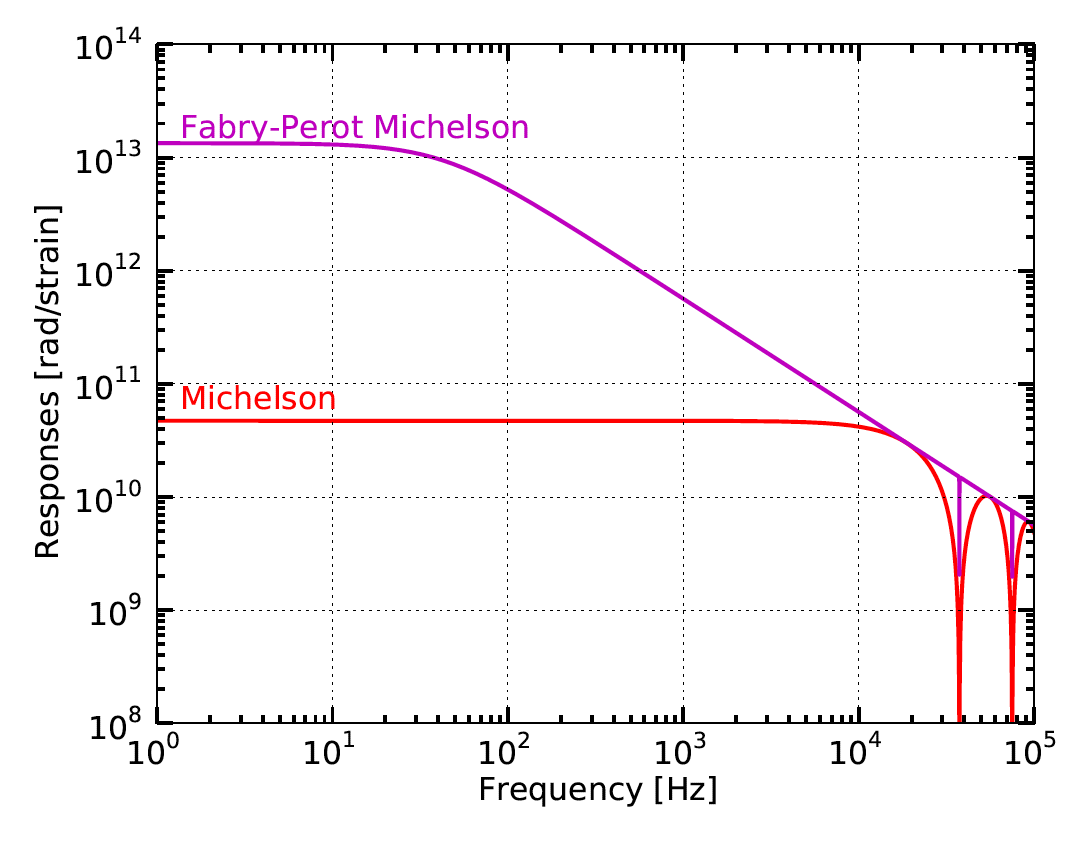
\includegraphics[width=10cm]{./response_mi-fpmi.png}
\end{center}


式(\ref{eq:eq8_})を$\omega_{\mathrm{g}}$の関数としてプロットしたものを図\ref{img:img1}に示す。まずDCでは$\frac{\omega_{\mathrm{g}}l}{c}\ll1$の条件をみたすので、DCゲインは
\begin{equation}
  |H_{\mathrm{MI(DC)}}|\sim\frac{2\omega_{0}l}{c}
\end{equation}
となる。つまり基線長が長くなればなるほど重力波への感度は向上する。
しかし高周波になると、
\begin{eqnarray}
  |H_{\mathrm{MI(AC)}}| \sim 2\frac{\omega_{0}}{\omega_{\mathrm{g}}}|\mathrm{sin}(\frac{\omega_{\mathrm{g}}l}{c})|
\end{eqnarray}
となって、1次で感度が悪くなる。これはMichelson干渉計で測る位相は重力波を時間積分しているためである。また
\begin{eqnarray}
  \mathrm{sin}(\frac{\omega_{\mathrm{g}}l}{c})=0 &\Leftrightarrow& \omega_{\mathrm{g}} = \pi\frac{c}{l}n, \, (nは整数)\\
 &\Leftrightarrow& \lambda_{\mathrm{g}} = \frac{l}{2} n, \,(\lambda_{\mathrm{g}} \equiv 2\pi{c}/\omega_{\mathrm{g}})
\end{eqnarray}
という条件では、ゲインが0になってしまい感度を持たないことがわかる。これは重力波の波長$\lambda_{\mathrm{g}}$が基線長の半整数倍のとき、BSとエンドミラーは節になって動いていないように見えるためである。
カットオフ周波数$f$は、$\mathrm{sin}(\frac{\omega_{\mathrm{g}}l}{c})=1$とすれば、
\begin{eqnarray}
  2\frac{\omega_{0}}{\omega_{\mathrm{g}}} &=& 2\frac{\omega_{0}l}{c}\mathrm{sin}(\frac{\omega_{\mathrm{g}}l}{c})=2\frac{\omega_{0}l}{c} \\
  \rightarrow f_{\mathrm{g}} &=& \frac{c}{2\pi{l}}
\end{eqnarray}
となり、基線長が長くなればなるほどカットオフ周波数が小さくなり、帯域が狭くなることがわかる。したがって観測帯域を$1\,\mathrm{kHz}$まで取るには、$50\, \mathrm{km}$まで伸ばす必要がある。このような長基線は現実的ではないので、FabryPerot共振器をつかって実行的な腕の長さを伸ばした、Michelson干渉計がつかわれている。


\subsection{腕をFabry-Perot共振器にしたときの応答}

\begin{center}
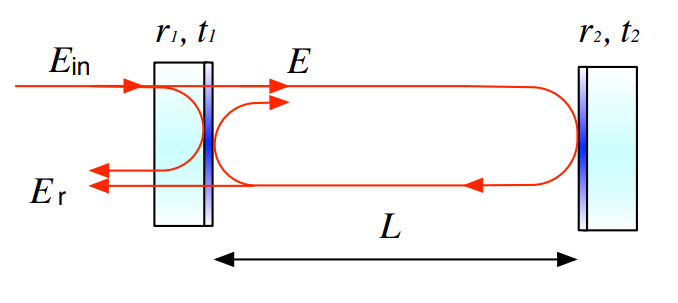
\includegraphics[width=10cm]{./FPcavity.png}
\end{center}

図より,共振器内部の電場$E(t)$と反射光の電場$E_{r}(t)$は以下のように関係している。
\begin{eqnarray}
  E(t) = t_{1}E_{in} + r_{1}r_{2}E(t-2T)e^{-i\Delta{\phi(t)}}, \\\label{eq:eq9}
  E_{r}(t) = -r_{1}E_{in} + r_{2}t_{1}E(t-2T)e^{-i\Delta{\phi(t)}},\\\label{eq:eq10}
  \Delta\phi(t) = \frac{\omega_{0}}{2}\int_{t-2L/c}^{t} h(t^{\prime})\, dt^{\prime} \label{eq:eq11}
\end{eqnarray}
ここで$\Delta{\phi(t)}$は共振器を往復したときに生じる位相差であり,式(\ref{eq:eq5})と同様にして計算した。


さて共振器内の電場$E(t)$のゆらぎを考えてみる。
\begin{equation}
  E(t) = \overline{E} + \delta{E(t)}
\end{equation}
のように表し、$\Delta\phi(t)$が十分に小さいとすれば、式(\ref{eq:eq9})は
\begin{equation}
\boxed{}
\end{equation}



Fabry-Perot共振器を大きな一枚の鏡だとみなしてみる。反射光の位相遅れ$Delta_{\phi_{r}}(\omega)$は,
\begin{equation}
\Delta_{\phi_{r}(\omega)} \equiv \frac{\delta{E_{r}}(\omega)}{\overline{E_{r}}} = 
\end{equation}
となる。


このFabry-Perot共振器を腕にもったMichelson干渉計の,重力波の応答は
\begin{equation}
\boxed{H_{FPMI}(\omega) \equiv \frac{2\Delta{\phi_{r}(\omega)}}{h(\omega)} = \frac{t_{1}^{2}r_{2}}{(t_{1}^{2}+r_{1}^{2})r_{2}-r_{1}}\frac{H_{MI}(\omega)}{1-r_{1}r_{2}\mathrm{exp}(-2i\omega{L}/c)}}
\end{equation}
である。

\subsection{Fabry-Perot共振器の応答}
\subsubsection{周波数への応答}
入射光の周波数が揺らいだときに,共振器内部の周波数がどのようにゆらぐのかもとめる。まず入射光を
\begin{equation}
E_{in}(t) = Ae^{i\Psi(t)}
\end{equation}
のように表す。$\Psi(t)$は入射光の周波数ゆらぎから生じる位相ゆらぎを表している。このゆらぎが十分に小さい場合.....
内部パワーのゆらぎ$\delta{E(t)}$は
\begin{equation}
\delta{E(s)} = i \frac{t_{1}A}{1-r_{1}r_{2}e^{-2sT}}\Psi(a)
\end{equation}
となる。共振器内部で生じる位相遅れ$\Delta{\phi(s)}$は,
\begin{equation}
\Delta{\phi_{f}(\omega)} \equiv -i \frac{\delta{E}(\omega)}{\overline{E}} = \frac{1-r_{1}r_{2}}{1-r_{1}r_{2}e^{-2sT}}\Psi{(s)} 
\end{equation}
となる。
さらに,周波数ゆらぎは位相ゆらぎを微分すればもとまるので,入射光の周波数ゆらぎを$\Delta{\nu_{laser}}\equiv -i(s/2\pi)\Psi$と定義し,$\Delta{\nu}\equiv -i(s/2\pi)\Delta\phi$と定義すると,入射光の周波数ゆらぎから共振器内部で生じる周波数ゆらぎへの応答は
\begin{equation}
 \boxed{C(s) = \frac{\Delta\nu}{\Delta\nu_{laser}} = \frac{1-r_{1}r_{2}}{1-r_{1}r_{2}e^{-2sT}}}
\end{equation}
となる。
